\documentclass[11pt]{article}
% For reading variables from external file
\usepackage{caption} 
\usepackage{subcaption} 
\usepackage{natbib} 
\usepackage{datatool}
\usepackage{cleveref} 
\usepackage{amsmath} 
\usepackage{graphicx}
\usepackage{parskip} 
\usepackage[margin=1.5cm]{geometry} 
\DTLsetseparator{,}



\begin{document}
\pagenumbering{gobble}
% Usage: \dat{variable-name}
%   This prints the value of the variable to the document
\DTLloaddb[noheader, keys={thekey,thevalue}]{dat}{../data/derived/report-summary-data.csv}
\newcommand{\dat}[1]{\DTLfetch{dat}{thekey}{#1}{thevalue}}

\section*{Estimating the magnitude of completion based on data recorded between \dat{date_start} and \dat{date_now}}%
\label{sec:Estimating the magnitude of completion}

We assume the magnitude $m$ of an earthquake is exponentially distributed
with parameter $\beta$. The frequency of earthquakes at a particular magnitude $m$,
denoted $N(m)$, will then be proportional to the exponential probability density function, that is:
\begin{equation}
    N(m) \propto \beta e^{-\beta m}.
\end{equation}
Taking logs, we get
\begin{equation}\label{eq:mod}
    \log N(m) = \underbrace{\alpha\beta}_{a}-\underbrace{\beta}_b\cdot m,
\end{equation}
which is a linear model with an intercept and linear term: $\log N(m)=a-bm$, where $a$ and $b$
are unknown coefficients.

To estimate $m_c$, we use a method proposed by \cite{wiemer}.
First, the magnitudes are binned, where $N(m)$ denotes the frequency
counts for the bin with lower limit $m$.
The bin-width is set to \dat{bin_width}.
The candidate values $M_1,\dots,M_{max}$ for $m_c$ are then iterated, and the linear model
in \cref{eq:mod} is fitted to the subset of data with magnitudes equal to or
greater than $M_j$. The goodness of fit of a candidate $M_j$, 
with corresponding parameter estimates $(\hat{a}, \hat{b})$,
 is given by
 \begin{equation}\label{eq:goodness}
    R(\hat{a},\hat{b},M_j)=100 - 100 \left( \frac{\sum_{M_i=M_j}^{M_{max}} |B_i - S_i|}{\sum_{M_i=M_j}^{M_{max}} B_i}  \right),
\end{equation}
where $B_i$ is the cumulative count of bins with magnitude $M_i$ or lower, and $S_i$ is
the corresponding cumulative count predicted by the fitted linear model.
The results are shown in \cref{fig:goodness}, and we pick the smallest $m_c$ candidate
that achieves a goodness of fit above \dat{explained_variance}\%.
This gives
\begin{equation}
    \widehat{m_c}=\dat{mc},
\end{equation}
when only using data from the last 12 months. The corresponding model fit
parameters are $\hat{a}=\dat{a_hat}$ and $\hat{b}=\dat{b_hat}$, for which the
data for the past 12 months is plotted in a histogram in \cref{fig:hist} along
with the predictions.  We see that above $m_c=\dat{mc}$, the magnitudes are
approximately exponentially distributed, although there are only
\dat{num_complete_observations} earthquakes with magnitudes above this level,
so there is uncertainty involved.

\begin{figure}[htp]
\centering
\begin{subfigure}[b]{0.49\textwidth}
    \centering
    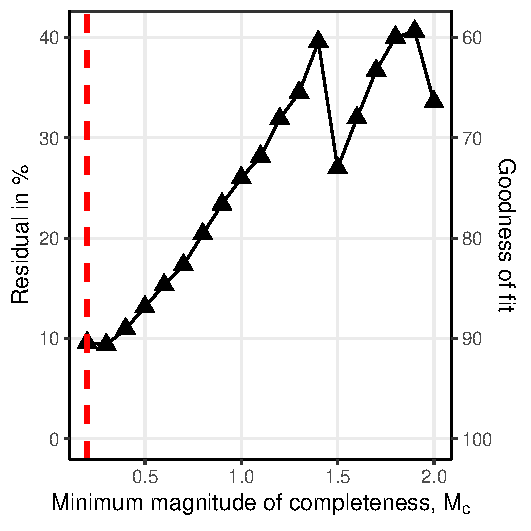
\includegraphics[scale=1.0]{../outputs/figures/goodness-of-fit.pdf}
    \caption{The goodness of fit for each candidate value $M_j$ for $m_c$, according to \cref{eq:goodness},
        with the selected value highlighted.
   }
    \label{fig:goodness}
\end{subfigure}
\hfill
\begin{subfigure}[b]{0.49\textwidth}
    \centering
    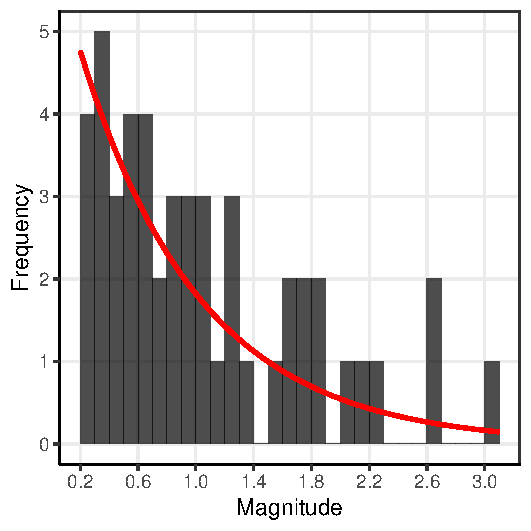
\includegraphics[scale=1.0]{../outputs/figures/earthquake-histogram.pdf}
    \caption{Earthquake frequencies for magnitudes $m\geq m_c=\dat{mc}$ in the past 12 months. The histogram bin width is \dat{bin_width}.}
    \label{fig:hist}
\end{subfigure}
\caption{Goodness of fit metrics for different magnitudes of completeness, along with an exponential fit
to the data above the selected value.}
\label{fig:figs1}
\end{figure}

\newpage

% Read month from data and change dynamically
\section*{Earthquake activity in \dat{month_now}}%

\begin{figure}[htp]
\begin{center}
    \includegraphics[scale=1]{../outputs/figures/earthquake-map.pdf}
\end{center}
\caption{Map of Northern Netherland, overlayer with the epicentres of the earthquakes recorded in the past 12 months.
The size of the circles correspond to the earthquakes' magnitude.}
\label{fig:map}
\end{figure}

\begin{figure}[htp]
\begin{center}
    \includegraphics[scale=1]{../outputs/figures/earthquake-hist.pdf}
\end{center}
\caption{Histogram of the magnitudes of the earthquakes recorded in the past 12 months.}
\label{fig:hist}
\end{figure}

In \dat{month_now}, there were \dat{count_last_month} earthquakes recorded above magnitude
$m_c=\dat{mc}$. In the 11 preceding months, there were \dat{count_11_month}, with an average monthly
count of \dat{avg_count_11_month}, meaning there was less earthquakes than expected last month.
The largest magnitude was \dat{max_last_month}, compared to a magnitude \dat{max_11_month} earthquake that
happened in the 11 months prior. The distribution of the earthquakes is shown in \cref{fig:hist}, with the
average magnitude being \dat{mean_last_month} in the last month and \dat{mean_11_month} in the preceding 11 months.
The location of all the earthquakes in the past 12 months is shown in \cref{fig:map}.
We see that both of the earthquakes last month happened in the same location, close to where most of the earthquakes in the
11 months preceding happened as well.


% Estimate Mc using
%
% Minimum Magnitude of Completeness in Earthquake Catalogs:
% Examples from Alaska, the Western United States, and Japan
% by Stefan Wiemer and Max Wyss (see earthquakes in DOwnloads)
%
% https://agupubs.onlinelibrary.wiley.com/doi/full/10.26464/epp2018015?saml_referrer
%
% https://agupubs.onlinelibrary.wiley.com/doi/full/10.26464/epp2018015?saml_referrer
%
% Need to figure out how to perform the estimation again, because don't get working plots...
%
% summary here...
%
% https://pubs.geoscienceworld.org/ssa/bssa/article/90/4/859/120531/Minimum-Magnitude-of-Completeness-in-Earthquake
%
% Use this ^^ ?
%
% Downloads/CORSSA as well...
%
% When get back, just try to make the estimate as simple as possible i.e. just use idea of shifting data by Mc and then using exponential MLE or something and use a different metric to measure goodness of fit, for example binned MSE or something, averaged over number of "predictions" made instead of sum over true values...




% TODO plan
% * create driver script for Q2 on MCMC, and make the plots nice
% * Write report for it, with conclusion

\bibliographystyle{unsrtnat}
\bibliography{references}

\end{document}
